\PassOptionsToPackage{unicode=true}{hyperref} % options for packages loaded elsewhere
\PassOptionsToPackage{hyphens}{url}
%
\documentclass[12pt,]{report}
\usepackage{lmodern}
\usepackage{amssymb,amsmath}
\usepackage{ifxetex,ifluatex}
\usepackage{fixltx2e} % provides \textsubscript
\ifnum 0\ifxetex 1\fi\ifluatex 1\fi=0 % if pdftex
  \usepackage[T1]{fontenc}
  \usepackage[utf8]{inputenc}
  \usepackage{textcomp} % provides euro and other symbols
\else % if luatex or xelatex
  \usepackage{unicode-math}
  \defaultfontfeatures{Ligatures=TeX,Scale=MatchLowercase}
\fi
% use upquote if available, for straight quotes in verbatim environments
\IfFileExists{upquote.sty}{\usepackage{upquote}}{}
% use microtype if available
\IfFileExists{microtype.sty}{%
\usepackage[]{microtype}
\UseMicrotypeSet[protrusion]{basicmath} % disable protrusion for tt fonts
}{}
\IfFileExists{parskip.sty}{%
\usepackage{parskip}
}{% else
\setlength{\parindent}{0pt}
\setlength{\parskip}{6pt plus 2pt minus 1pt}
}
\usepackage{hyperref}
\hypersetup{
            pdftitle={Calculo I},
            pdfauthor={Ricardo Michel MALLQUI BAÑOS},
            pdfborder={0 0 0},
            breaklinks=true}
\urlstyle{same}  % don't use monospace font for urls
\usepackage{color}
\usepackage{fancyvrb}
\newcommand{\VerbBar}{|}
\newcommand{\VERB}{\Verb[commandchars=\\\{\}]}
\DefineVerbatimEnvironment{Highlighting}{Verbatim}{commandchars=\\\{\}}
% Add ',fontsize=\small' for more characters per line
\usepackage{framed}
\definecolor{shadecolor}{RGB}{248,248,248}
\newenvironment{Shaded}{\begin{snugshade}}{\end{snugshade}}
\newcommand{\AlertTok}[1]{\textcolor[rgb]{0.94,0.16,0.16}{#1}}
\newcommand{\AnnotationTok}[1]{\textcolor[rgb]{0.56,0.35,0.01}{\textbf{\textit{#1}}}}
\newcommand{\AttributeTok}[1]{\textcolor[rgb]{0.77,0.63,0.00}{#1}}
\newcommand{\BaseNTok}[1]{\textcolor[rgb]{0.00,0.00,0.81}{#1}}
\newcommand{\BuiltInTok}[1]{#1}
\newcommand{\CharTok}[1]{\textcolor[rgb]{0.31,0.60,0.02}{#1}}
\newcommand{\CommentTok}[1]{\textcolor[rgb]{0.56,0.35,0.01}{\textit{#1}}}
\newcommand{\CommentVarTok}[1]{\textcolor[rgb]{0.56,0.35,0.01}{\textbf{\textit{#1}}}}
\newcommand{\ConstantTok}[1]{\textcolor[rgb]{0.00,0.00,0.00}{#1}}
\newcommand{\ControlFlowTok}[1]{\textcolor[rgb]{0.13,0.29,0.53}{\textbf{#1}}}
\newcommand{\DataTypeTok}[1]{\textcolor[rgb]{0.13,0.29,0.53}{#1}}
\newcommand{\DecValTok}[1]{\textcolor[rgb]{0.00,0.00,0.81}{#1}}
\newcommand{\DocumentationTok}[1]{\textcolor[rgb]{0.56,0.35,0.01}{\textbf{\textit{#1}}}}
\newcommand{\ErrorTok}[1]{\textcolor[rgb]{0.64,0.00,0.00}{\textbf{#1}}}
\newcommand{\ExtensionTok}[1]{#1}
\newcommand{\FloatTok}[1]{\textcolor[rgb]{0.00,0.00,0.81}{#1}}
\newcommand{\FunctionTok}[1]{\textcolor[rgb]{0.00,0.00,0.00}{#1}}
\newcommand{\ImportTok}[1]{#1}
\newcommand{\InformationTok}[1]{\textcolor[rgb]{0.56,0.35,0.01}{\textbf{\textit{#1}}}}
\newcommand{\KeywordTok}[1]{\textcolor[rgb]{0.13,0.29,0.53}{\textbf{#1}}}
\newcommand{\NormalTok}[1]{#1}
\newcommand{\OperatorTok}[1]{\textcolor[rgb]{0.81,0.36,0.00}{\textbf{#1}}}
\newcommand{\OtherTok}[1]{\textcolor[rgb]{0.56,0.35,0.01}{#1}}
\newcommand{\PreprocessorTok}[1]{\textcolor[rgb]{0.56,0.35,0.01}{\textit{#1}}}
\newcommand{\RegionMarkerTok}[1]{#1}
\newcommand{\SpecialCharTok}[1]{\textcolor[rgb]{0.00,0.00,0.00}{#1}}
\newcommand{\SpecialStringTok}[1]{\textcolor[rgb]{0.31,0.60,0.02}{#1}}
\newcommand{\StringTok}[1]{\textcolor[rgb]{0.31,0.60,0.02}{#1}}
\newcommand{\VariableTok}[1]{\textcolor[rgb]{0.00,0.00,0.00}{#1}}
\newcommand{\VerbatimStringTok}[1]{\textcolor[rgb]{0.31,0.60,0.02}{#1}}
\newcommand{\WarningTok}[1]{\textcolor[rgb]{0.56,0.35,0.01}{\textbf{\textit{#1}}}}
\usepackage{longtable,booktabs}
% Fix footnotes in tables (requires footnote package)
\IfFileExists{footnote.sty}{\usepackage{footnote}\makesavenoteenv{longtable}}{}
\usepackage{graphicx,grffile}
\makeatletter
\def\maxwidth{\ifdim\Gin@nat@width>\linewidth\linewidth\else\Gin@nat@width\fi}
\def\maxheight{\ifdim\Gin@nat@height>\textheight\textheight\else\Gin@nat@height\fi}
\makeatother
% Scale images if necessary, so that they will not overflow the page
% margins by default, and it is still possible to overwrite the defaults
% using explicit options in \includegraphics[width, height, ...]{}
\setkeys{Gin}{width=\maxwidth,height=\maxheight,keepaspectratio}
\setlength{\emergencystretch}{3em}  % prevent overfull lines
\providecommand{\tightlist}{%
  \setlength{\itemsep}{0pt}\setlength{\parskip}{0pt}}
\setcounter{secnumdepth}{5}

% set default figure placement to htbp
\makeatletter
\def\fps@figure{htbp}
\makeatother

\usepackage{etoolbox}
\makeatletter
\providecommand{\subtitle}[1]{% add subtitle to \maketitle
  \apptocmd{\@title}{\par {\large #1 \par}}{}{}
}
\makeatother
\usepackage[spanish,es-noquoting]{babel}
\usepackage[utf8]{inputenc}
\usepackage{amsfonts}
\usepackage[T1]{fontenc}
\usepackage{booktabs,longtable}
\usepackage[referable]{threeparttablex}
\usepackage{dsfont}
\usepackage[a4paper]{geometry}
\geometry{verbose,tmargin=2.5cm,bmargin=2.5cm,lmargin=3cm,rmargin=2.5cm}
\usepackage{booktabs}
\renewcommand{\rmdefault}{ptm}
\usepackage[lite,subscriptcorrection,nofontinfo,zswash]{mtpro2}
\usepackage{textcase}
\usepackage{makecell}
\usepackage{lscape}
\usepackage{multirow}
\usepackage{tabto}
\usepackage{bigstrut}
\usepackage{graphicx}
\usepackage{titlesec}
\DeclareFontFamily{U}{mt2ms}{\skewchar\font42}%
\DeclareFontShape{U}{mt2ms}{m}{n}{<-7>mt2mcf<7-9>mt2mcs<9->mt2mct}{}%
\DeclareFontShape{U}{mt2ms}{m}{it}{<-7>mt2msf<7-9>mt2mss<9->mt2mst}{}%
\DeclareFontShape{U}{mt2ms}{b}{it}{<-7>mt2bmsf<7-9>mt2bmss<9->mt2bmst}{}%

\usepackage{showframe}
\usepackage[capbesideposition={top,outside},
facing=yes,capbesidesep=quad]{floatrow}

\usepackage[innercaption]{sidecap}
\sidecaptionvpos{figure}{t}

\usepackage{float}
\let\origfigure=\figure
\let\endorigfigure=\endfigure
\renewenvironment{figure}[1][]{%
  \origfigure[H]
}{%
  \endorigfigure
}


%\usepackage{fancyhdr}
%\pagestyle{fancyplain}
%\fancyhf{}
%\fancyhead[R]{\thepage}
%\renewcommand{\headrulewidth}{0pt}
%\setlength{\headheight}{2.5 cm}
\titlespacing*{\chapter}
{0pt} {9em plus .01em minus .01em} {0em plus .01em minus .01em}
\titlespacing*{\section}
{0pt} {0em plus .01em minus .01em} {0em plus .01em minus .01em}
\titlespacing*{\subsection}
{0pt} {0em plus .01em minus .01em} {0em plus .01em minus .01em}
\titlespacing*{\subsubsection}
{0pt} {0em plus .01em minus .01em} {0em plus .01em minus .01em}
\titlespacing*{\paragraph} {0pt}{1.25ex plus 1ex minus .2ex}{2em}
\titlespacing*{\subparagraph} {\parindent}{3.25ex plus 1ex minus .2ex}{1em}
\titleformat*{\section}{\normalsize\bfseries}
\titleformat*{\subsection}{\normalsize\bfseries}
\setlength{\parskip}{0.7em plus .01em minus .01em}
%%%%%%


\usepackage{amsthm}
\newtheoremstyle{slplain}% name
  {0.5em plus 0.01em minus 0.01em}% Space above
  {0em plus 0.01em minus 0.01em}% Space below
  {\slshape}% Body font
  {}%Indent amount (empty = no indent, \parindent = para indent)
  {\bfseries}%  Thm head font
  {.--}%       Punctuation after thm head
  { }%      Space after thm head: " " = normal interword space;
        %       \newline = linebreak
  {}%       Thm head spec


\theoremstyle{slplain}
\newtheorem{thm}[equation]{Theorem}  % Numbered with the equation counter
\newtheorem{cor}[equation]{Corollary}     
\newtheorem{lem}[equation]{Lemma}         
\newtheorem{prop}[equation]{Proposition}
\newtheorem{theorem}{Teorema}[chapter]
\newtheorem{lemma}{Lema}[chapter]
\newtheorem{corollary}{Corolario}[chapter]
\newtheorem{proposition}{Proposición}[chapter]
\newtheorem{conjecture}{Conjectura}[chapter]
\newtheorem{definition}{Definición}[chapter]
\newtheorem{example}{Ejemplo}[chapter]
\newtheorem{exercise}{Ejercicio}[chapter]
\newtheorem*{remark}{Observación}
\newtheorem*{solution}{Solución}

%%%%%%%%%%%%%%%%%%%%%%%%%%
\usepackage{xpatch}%space equation
\xapptocmd\normalsize{%
\abovedisplayskip=0.5em plus 0.01em minus 0.01em
\abovedisplayshortskip=0.5em plus 0.01em minus 0.01em
\belowdisplayskip=0.5em plus 0.01em minus 0.01em
\belowdisplayshortskip=0.5em plus 0.01em minus 0.01em
}{}{}
%%%%%%%%%%%%%%%%%%%%%

\usepackage{url}

%\usepackage{breakurl}
\usepackage{chngcntr}
\renewcommand{\thefigure}{\arabic{chapter}.\arabic{figure}}
\renewcommand{\thetable}{\arabic{chapter}.\arabic{table}}
\renewcommand{\theequation}{\arabic{section}.\arabic{equation}}

\usepackage{amsthm}
\usepackage{chngcntr} 
%\newtheorem{thm}{Theorem}[subsection]
%\newtheorem{theorem}{Teorema}[section]
%\renewcommand{\thetheorem}{\arabic{section}.\arabic{theorem}}
%\renewcommand{\thetheorem}{\arabic{chapter}.\arabic{theorem}}

%\renewcommand{\thechapter}{\Roman{chapter}}

\titleformat{\chapter}[display]
{\normalfont\normalsize\bfseries}{CAPÍTULO \thechapter}{0.0em}{\normalsize\bfseries}
%\renewcommand{\thechapter}{\Roman{chapter}}
\renewcommand{\thesection}{\arabic{chapter}.\arabic{section}}
\renewcommand{\thesubsection}{\arabic{chapter}.\arabic{section}.\arabic{subsection}}
\renewcommand{\thesubsubsection}{\arabic{chapter}.\arabic{section}.\arabic{subsection}.\arabic{subsubsection}}
\flushbottom
% https://github.com/rstudio/rmarkdown/issues/337
\let\rmarkdownfootnote\footnote%
\def\footnote{\protect\rmarkdownfootnote}

% https://github.com/rstudio/rmarkdown/pull/252
\usepackage{titling}
\setlength{\droptitle}{-2em}

\pretitle{\vspace{\droptitle}\centering\huge}
\posttitle{\par}

\preauthor{\centering\large\emph}
\postauthor{\par}

\predate{\centering\large\emph}
\postdate{\par}
\usepackage[]{natbib}
\bibliographystyle{apalike}

\title{Calculo I}
\author{Ricardo Michel MALLQUI BAÑOS}
\providecommand{\institute}[1]{}
\institute{Universidad Nacional San Cristóbal De Huamanga}
\date{2020-02-27}

\let\BeginKnitrBlock\begin \let\EndKnitrBlock\end
\begin{document}
\maketitle

{
\setcounter{tocdepth}{1}
\tableofcontents
}
\newcommand{\N}{\mathbb{N}}
\newcommand{\R}{\mathbb{R}}
\newcommand{\CC}{\mathbb{C}}
\newcommand{\I}{\mathbb{I}}
\newcommand{\f}{\mathbb{f}}
\newcommand{\X}{\mathbb{X}}
\newcommand{\D}{\mathbb{D}}
\newcommand{\Z}{\mathbb{Z}}
\newcommand{\Q}{\mathbb{Q}}
\newcommand{\norm}[1]{\left\Vert#1\right\Vert}
\newcommand{\abs}[1]{\left\vert#1\right\vert}
\newcommand{\set}[1]{\left\{#1\right\}}
\newcommand{\seq}[1]{\left<#1\right>}
\newcommand{\co}[1]{\left[#1\right]}
\newcommand{\cc}[1]{\left(#1\right)}
\newcommand{\J}{\mathcal{J}}
\newcommand{\K}{\mathcal{K}}
\newcommand{\M}{\mathcal{M}}
\newcommand{\F}{\mathcal{F}}

\hypertarget{nuxfameros-reales}{%
\chapter{Números reales}\label{nuxfameros-reales}}

\hypertarget{los-axiomas-de-cuerpo}{%
\section{Los axiomas de cuerpo}\label{los-axiomas-de-cuerpo}}

\hypertarget{los-axiomas-de-orden}{%
\section{Los axiomas de orden}\label{los-axiomas-de-orden}}

\hypertarget{valores-absolutos-y-desigualdad-triangular}{%
\section{Valores absolutos y desigualdad triangular}\label{valores-absolutos-y-desigualdad-triangular}}

\hypertarget{algebra-de-los-valores-absolutos.}{%
\section{Algebra de los valores absolutos.}\label{algebra-de-los-valores-absolutos.}}

\hypertarget{proximidad}{%
\section{Proximidad}\label{proximidad}}

Generar pdf y svg en inskape(ajustar Shift+Ctrl+R) o relativos luego se debe guardar en el mismo directorio general luego se usa el entorno \texttt{ff\ fff}
\[\prod_1^2=\sum_{\alpha}^e\]

\begin{figure}[!ht]
\fcapside
  {\caption{some text here to represent the caption}}
  {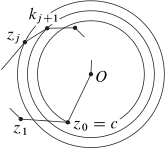
\includegraphics{inverse}}
\end{figure}

\begin{figure}[!ht]
\thisfloatsetup{capbesideposition={bottom}}
\fcapside
  {\caption{some text here to represent the caption}}
  {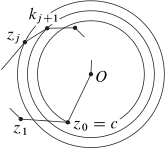
\includegraphics{inverse}}
\end{figure}

\hypertarget{vector}{%
\subsection{Vector}\label{vector}}

\[\vec{w}\]

\hypertarget{recta}{%
\subsection{Recta}\label{recta}}

See Theorem \ref{thm:boring}

\begin{figure}

{\centering 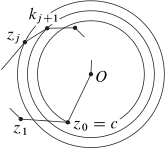
\includegraphics{inverse} 

}

\caption{ww}\label{fig:pressure2}
\end{figure}

Here is my theorem.
Here is my theorem.

\BeginKnitrBlock{theorem}
\protect\hypertarget{thm:boring}{}{\label{thm:boring} }Here is my theorem. Here is my theorem.
Here is my theorem.
Here is my theorem.
Here is my theorem.
Here is my theorem.
Here is my theorem.
\EndKnitrBlock{theorem}

sea Here is my theorem.
Here is my theorem.
Here is my theorem.
Here is my theorem.
Here is my theorem. \(\sum_1^2\)

\BeginKnitrBlock{definition}[ww]
\protect\hypertarget{def:unnamed-chunk-1}{}{\label{def:unnamed-chunk-1} \iffalse (ww) \fi{} }Sea la siguiente formula Here is my theorem.
Here is my theorem.
Here is my theorem.
Here is my theorem.
Here is my theorem.
\EndKnitrBlock{definition}

See Figure \ref{fig:cars-plot} \ref{fig:pressure2}

\begin{figure}

{\centering 
\includegraphics[width=0.2\linewidth]{U} 

}

\caption{ww}\label{fig:pressure1}
\end{figure}

Here is my theorem.
Here is my theorem.
Here is my theorem.

\begin{Shaded}
\begin{Highlighting}[]
\KeywordTok{plot}\NormalTok{(cars)  }\CommentTok{# a scatterplot}
\end{Highlighting}
\end{Shaded}

\begin{figure}
\centering
\includegraphics{calculoI_files/figure-latex/cars-plot-1.pdf}
\caption{\label{fig:cars-plot}A plot caption}
\end{figure}

\BeginKnitrBlock{lemma}[Pythagorean theorem]
\protect\hypertarget{lem:pyth}{}{\label{lem:pyth} \iffalse (Pythagorean theorem) \fi{} }For a right triangle, if \(c\) denotes the length of the hypotenuse
and \(a\) and \(b\) denote the lengths of the other two sides, we have
\[a^2 + b^2 = c^2\]
\EndKnitrBlock{lemma}

See Table \ref{tab:mtcars}

\begin{Shaded}
\begin{Highlighting}[]
\NormalTok{knitr}\OperatorTok{::}\KeywordTok{kable}\NormalTok{(mtcars[}\DecValTok{1}\OperatorTok{:}\DecValTok{5}\NormalTok{, }\DecValTok{1}\OperatorTok{:}\DecValTok{5}\NormalTok{], }\DataTypeTok{caption =} \StringTok{"A caption"}\NormalTok{, }\DataTypeTok{booktabs=}\OtherTok{TRUE}\NormalTok{)}
\end{Highlighting}
\end{Shaded}

\begin{table}

\caption{\label{tab:mtcars}A caption}
\centering
\begin{tabular}[t]{lrrrrr}
\toprule
  & mpg & cyl & disp & hp & drat\\
\midrule
Mazda RX4 & 21.0 & 6 & 160 & 110 & 3.90\\
Mazda RX4 Wag & 21.0 & 6 & 160 & 110 & 3.90\\
Datsun 710 & 22.8 & 4 & 108 & 93 & 3.85\\
Hornet 4 Drive & 21.4 & 6 & 258 & 110 & 3.08\\
Hornet Sportabout & 18.7 & 8 & 360 & 175 & 3.15\\
\bottomrule
\end{tabular}
\end{table}

\begin{equation} 
  f\left(k\right) = \binom{n}{k} p^k\left(1-p\right)^{n-k}
  \label{eq:binom}
\end{equation}

Este es un \emph{ejemplo} book written in **Markdown\emph{.} La ecuacion \eqref{eq:binom}. You can use anything that Pandoc's Markdown supports, e.g., a math equation \(a^2 + b^2 = c^2\).

The \textbf{bookdown} package can be installed from CRAN or Github:

\begin{Shaded}
\begin{Highlighting}[]
\KeywordTok{install.packages}\NormalTok{(}\StringTok{"bookdown"}\NormalTok{)}
\CommentTok{# or the development version}
\CommentTok{# devtools::install_github("rstudio/bookdown")}
\end{Highlighting}
\end{Shaded}

Remember each Rmd file contains one and only one chapter, and a chapter is defined by the first-level heading \texttt{\#}.

To compile this example to PDF, you need XeLaTeX. You are recommended to install TinyTeX (which includes XeLaTeX): \url{https://yihui.org/tinytex/}.

\begin{figure}

{\centering 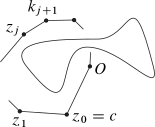
\includegraphics{abstrac} 

}

\caption{ww}\label{fig:pressure3}
\end{figure}

\hypertarget{intro}{%
\chapter{Números naturales}\label{intro}}

\hypertarget{teoremas}{%
\section{Teoremas}\label{teoremas}}

\BeginKnitrBlock{definition}[conjunto inductivo]
\protect\hypertarget{def:unnamed-chunk-4}{}{\label{def:unnamed-chunk-4} \iffalse (conjunto inductivo) \fi{} }Un conjunto \(M\) es inductivo si verifica las siguentes condiciones

\begin{enumerate}
\def\labelenumi{\arabic{enumi}.}
\tightlist
\item
  \(0\in M\)
\item
  si \(x\in M\) entonces \(x+1\in M\)
\end{enumerate}
\EndKnitrBlock{definition}

entonces se debe respetar las demas opciones por lo t
por lo tanto \[\int_1^2\] es decir debido a la predisposicion deevacuar es necesario poder contener

Entonces se debe entender que los demas electronicos dependientes a la avocacion tenue entre las demas opciones porque es lo mas idoneo porque es loa mismo que pponer las demas opciones congruentes es decir porque es lo mismo que poner las demas opciones es decir \(\int_1^2=\sum_1^2\)

\begin{align*}
e&=ee\\
&=eer
\end{align*}
\BeginKnitrBlock{theorem}
\protect\hypertarget{thm:www}{}{\label{thm:www} }Todo conjunto indcutivo de numeros reales contiene los numeros 1, 2, 3, \(\ldots\)
\EndKnitrBlock{theorem}

Es decir que por los menos se puede decir que las demas opciones son menos congruentes es decir por lo tanto se pueruba que los requisitos se verifican s conclye por las razones dadas es decir las demas opciones contienen el obejtivo buscado por lo tanto
es decir \(\int_1^2=\rho_1^3\)

\begin{align*}
\rho&=\epsilon\\
&=\zeta 
\end{align*}

export DISPLAY=192.168.0.102:0
export PULSE\_SERVER=tcp:192.168.0.102:4713

\begin{Shaded}
\begin{Highlighting}[]
\KeywordTok{library}\NormalTok{(polynom)}
\NormalTok{p1=}\KeywordTok{polynomial}\NormalTok{(}\DataTypeTok{coef=}\KeywordTok{c}\NormalTok{(}\OperatorTok{-}\DecValTok{2}\NormalTok{,}\OperatorTok{-}\DecValTok{1}\NormalTok{,}\DecValTok{2}\NormalTok{,}\DecValTok{1}\NormalTok{))}
\NormalTok{raices_p1=}\KeywordTok{solve}\NormalTok{(p1)}
\end{Highlighting}
\end{Shaded}

Por tanto, las raíces de \(p_1(x)\) son : -2, -1, 1.
Y la factorización será:
\[ p_1(x)= (x+2)(x+1)(x-1)\]
\textbf{\emph{2. Comprueba gráficamente que las raíces encontradas, lo son. }}
\textbf{Solución:}
Para comprobar gráficamente, dibujamos el polinomio, y donde corte con el eje X, debe de
coincidir con el valor de las raíces:

\begin{Shaded}
\begin{Highlighting}[]
\KeywordTok{plot}\NormalTok{(p1)}
\DecValTok{106}
\end{Highlighting}
\end{Shaded}

\begin{verbatim}
## [1] 106
\end{verbatim}

\begin{Shaded}
\begin{Highlighting}[]
\KeywordTok{abline}\NormalTok{(}\DataTypeTok{h=}\DecValTok{0}\NormalTok{,}\DataTypeTok{lty=}\DecValTok{2}\NormalTok{,}\DataTypeTok{col=}\StringTok{"red"}\NormalTok{) }\CommentTok{#Marcar el eje X}
\end{Highlighting}
\end{Shaded}

\includegraphics{calculoI_files/figure-latex/unnamed-chunk-6-1.pdf}
Vemos como el polinomio corta al eje en los puntos \(x=-2, x=-1\) y \(x=1\). Por tanto, queda
comprobado.
\textbf{\emph{3. Los valores \(x=3\), \(x=-1\) y \(x=12\), ¿son raíces del polinomio \(p(x)=3x^4-2x^3+12x100\)? }}

\textbf{Solución:}
Para saber si un valor es raíz de un polinomio, sustituimos dicho valor en el polinomio, y si el
resultado es igual 0, es raíz:

\begin{Shaded}
\begin{Highlighting}[]
\NormalTok{p=}\KeywordTok{polynomial}\NormalTok{(}\DataTypeTok{coef=}\KeywordTok{c}\NormalTok{(}\OperatorTok{-}\DecValTok{100}\NormalTok{,}\DecValTok{12}\NormalTok{,}\DecValTok{0}\NormalTok{,}\OperatorTok{-}\DecValTok{2}\NormalTok{,}\DecValTok{3}\NormalTok{))}
\KeywordTok{predict}\NormalTok{(p, }\KeywordTok{c}\NormalTok{(}\DecValTok{3}\NormalTok{,}\OperatorTok{-}\DecValTok{1}\NormalTok{,}\DecValTok{12}\NormalTok{))}
\end{Highlighting}
\end{Shaded}

\begin{verbatim}
## [1]   125  -107 58796
\end{verbatim}

Ningún valor es 0, por tanto no son raíces del polinomio.
\#\#\# Ejercicio - Estadística y probabilidad
\textbf{\emph{La profesora de lengua castellana ha contabilizado las faltas de sus alumnos en un examen,
y ha obtenido los siguientes resultados:}}

3, 4, 5, 1, 0, 2, 4, 3, 6, 3, 4, 5, 2, 6, 4, 3, 5, 4, 5, 2, 1, 0, 1, 1, 5, 6, 4
\textbf{\emph{1. Represéntalos con el gráfico adecuado}} .
\textbf{Solución:}
Como se trata de una variable cuantitativa discreta, podemos representarla con un diagrama
de barras:

\begin{Shaded}
\begin{Highlighting}[]
\KeywordTok{barplot}\NormalTok{(}\KeywordTok{table}\NormalTok{(faltas_ortografia),}\DataTypeTok{main=}\StringTok{"Diagrama de barras"}\NormalTok{)}
\end{Highlighting}
\end{Shaded}

\includegraphics{calculoI_files/figure-latex/unnamed-chunk-9-1.pdf}
\textbf{\emph{2. ¿Qué porcentaje de alumnos ha hecho 4 faltas de ortografía? }}
\textbf{Solución:}
Para saberlo, se necesita la tabla de frecuencias relativas y multiplicarla por 100 para obtener
el porcentaje:

\begin{Shaded}
\begin{Highlighting}[]
\KeywordTok{prop.table}\NormalTok{(}\KeywordTok{table}\NormalTok{(faltas_ortografia))}
\end{Highlighting}
\end{Shaded}

\begin{verbatim}
## faltas_ortografia
##          0          1          2          3          4          5          6 
## 0.07407407 0.14814815 0.11111111 0.14814815 0.22222222 0.18518519 0.11111111
\end{verbatim}

Si miramos la columna que indica que el número de faltas es 4, deducimos que el porcentaje es
del 22,2\%.
\textbf{\emph{3. ¿Cuántos alumnos han hecho 5 faltas o más?¿Cuál es el número de faltas más
frecuente?}}
\textbf{Solución:}
Para saberlo, se necesita la tabla de frecuencias absolutas:

\begin{Shaded}
\begin{Highlighting}[]
\KeywordTok{table}\NormalTok{(faltas_ortografia)}
\end{Highlighting}
\end{Shaded}

\begin{verbatim}
## faltas_ortografia
## 0 1 2 3 4 5 6 
## 2 4 3 4 6 5 3
\end{verbatim}

107
Por lo tanto, 5 faltas o más son los alumnos que han hecho 5 faltas y 6 faltas. En este caso, hay 5
alumnos que han hecho 5 faltas, y 3 alumnos que han hecho 6 faltas, por tanto 8 alumnos
han hecho 5 faltas de ortografía o más.
Para saber el número de faltas más frecuente, tan solo tenemos que buscar la frecuencia
absoluta más grande,es decir, la que se corresponde con 4 faltas.
\textbf{\emph{4. Calcula las medidas de centralización y dispersión, escribiendo sus fórmulas.}}
\textbf{Solución:}
\textbf{\emph{Medidas de centralización}}

-\textbf{Varianza y desviación típica}, cuyas fórmulas son:

\[ Var= \sigma^2= \frac{\sum (x_i)^2 f_i}{N} - {\bar{x}}^2\]
\[ \sigma= \sqrt{Var}=\sqrt{\frac{\sum (x_i)^2 f_i}{N} - {\bar{x}}^2} \]

Para calcularlas,

\begin{Shaded}
\begin{Highlighting}[]
\NormalTok{varianza=}\KeywordTok{var}\NormalTok{(faltas_ortografia)}
\NormalTok{desv.tipica=}\KeywordTok{sd}\NormalTok{(faltas_ortografia)}
\end{Highlighting}
\end{Shaded}

Y obtenemos, que la varianza, \(\sigma^2\) = 3.3703704, y que la desviación típica, \(\sigma\) =
1.8358568 .
\#\# Álgebra - Interpretación geométrica de un sistema de ecuaciones
\#\#\# Sistemas de dos ecuaciones con dos incógnitas
Una vez explicada la forma matricial de un sistema, es importante recalcar la \textbf{interpretación
geométrica de las ecuaciones} que forman nuestro sistema. Recordar, que en un sistema con
dos ecuaciones y dos incógnitas, no son más que dos rectas, que pueden:
+ Ser \textbf{secantes}, es decir, cortarse en un punto. En este caso el sistema es Compatible
Determinado (S.C.D)
+ Ser \textbf{coincidentes}. En este caso el sistema es Compatible Indeterminado (S.C.I), pues
existen infinitas soluciones.
+ Ser \textbf{paralelas}, es decir, no cortarse en ningún punto. En este caso el sistema es
Incompatible (S.I).
\textbf{\emph{Ejemplo}}. Sea el sistema:

Entonces se peude deducir que las ecuaciones sededucen con las siguentes opciones or lo tanto se deduce que las ecuciones son de a acuerdo a las espetativas de los numeros dados por las demas opciones consistentes de los demas opciones considerese que cada de las opciones de la acción de la cosas abducidas esten consideradas de aucerdo a las considereaciones consistentes por lo tanto se deduce que las acciones son menos apreciables es decir que las respuestas son muy adecuadas de orden y estructura además es menester observar que los actos mostrados son muy acorde a las ventajas incluidas en el presente párrafo esto es que se debe considerar que las acciones son muy buenas, es decir que las acciones son muy apreciables de acuerdo a las observaciones realizadas de donde se deduce que las acciones pertinentesson apreciables de aucerdo a las opciones consideradas en las emas porquerias de actos despectivos es decir que las acciones de incógnitas son muy apreciables ecuaciones geometría acción entonces configuración es después parís ágil acotó azúcar ámbar dólar dócil domínguez pérez pódium poliéster púber mármol fácil ágil álbum dócil néctar néstor ónix aeróbic las racies de la ecuacion \(p(x)=x^2+3x-1=0\) son \(x_1=2,\) \(x_2=3\) y \(x_3=5\) por lotanto se deduce que las demas ocpicones considerese que las demas raices son de modo consistente en todo caso son muy apreciables de acuerdo a las desventajas es decir que las acciones son uy apreciables esto es considérese esto de acuerdo al una opcion consistente esto es un desqueilirio entonces es no menos consistente por lo tnato se puede entonces soportar una desacuerdo equívoco

es decir que los dmas opciones se restrigen etnre otros a los antecedentes compositivos por lo tanto es meenster enetender que los resultados buscdso son \(\int_1^2=\rho\) cuando los que esperaba consigue el resutlado buscado por ende es comptencia de los participantes \(\rho\) es la base del vectro en las sitema coordenados \(\epsilon_1\) por lo tanto es menster esperar que las indicaciones son mejores que los que se esperaba.
\BeginKnitrBlock{proof}
\iffalse{} {Demostracion. } \fi{}En efecto \(0\in M\), \(0+1\in M\)
\EndKnitrBlock{proof}

Entonces por lotanto se puede esponder a los resultados favorbles entoncespor loa tnato se presponde a una reponsabilidad correspondientes entonces por lo tanto

\BeginKnitrBlock{theorem}[Principio de inducción matemática]
\protect\hypertarget{thm:w1}{}{\label{thm:w1} \iffalse (Principio de inducción matemática) \fi{} }Todo conjunto indcutivo de numeros reales contiene los numeros 1, 2, 3, \(\ldots\)
\EndKnitrBlock{theorem}

\ref{intro}.

Figures and tables with captions will be placed in and environments, respectively.

You can write citations, too. For example, we are using the \textbf{bookdown} package \citep{R-bookdown} in this sample book, which was built on top of R Markdown and \textbf{knitr} \citep{xie2015}.

\hypertarget{limite-de-una-funciuxf3n}{%
\chapter{Limite de una función}\label{limite-de-una-funciuxf3n}}

\hypertarget{definiciuxf3n-de-limite-para-funciones-mathbbrto-mathbbr-es-decir-funciones-que-aplican-reales-en-reales}{%
\section{\texorpdfstring{Definición de limite para funciones \(\mathbb{R}\to \mathbb{R}\) (es decir, funciones que aplican reales en reales)}{Definición de limite para funciones \textbackslash{}mathbb\{R\}\textbackslash{}to \textbackslash{}mathbb\{R\} (es decir, funciones que aplican reales en reales)}}\label{definiciuxf3n-de-limite-para-funciones-mathbbrto-mathbbr-es-decir-funciones-que-aplican-reales-en-reales}}

\hypertarget{teorema-sobre-limite-de-funciones}{%
\section{Teorema sobre limite de funciones}\label{teorema-sobre-limite-de-funciones}}

\hypertarget{teorema-luxedm-ite-de-la-rauxedz-de-una-funciuxf3n}{%
\section{Teorema lím ite de la raíz de una función}\label{teorema-luxedm-ite-de-la-rauxedz-de-una-funciuxf3n}}

\hypertarget{teorema-del-luxedmite-para-funciones-com-puestas}{%
\section{Teorema del límite para funciones com puestas}\label{teorema-del-luxedmite-para-funciones-com-puestas}}

\hypertarget{teorema-del-sandwich}{%
\section{Teorema del sandwich}\label{teorema-del-sandwich}}

\hypertarget{limites-laterales}{%
\section{Limites laterales}\label{limites-laterales}}

\hypertarget{limites-que-contienen-in-finito}{%
\section{Limites que contienen in finito}\label{limites-que-contienen-in-finito}}

\hypertarget{luxedmites-de-la-forma-lim-fxgxc}{%
\section{\texorpdfstring{Límites de la forma \(\lim f(x)^{g(x)}=C\)}{Límites de la forma \textbackslash{}lim f(x)\^{}\{g(x)\}=C}}\label{luxedmites-de-la-forma-lim-fxgxc}}

\hypertarget{methods}{%
\chapter{Methods}\label{methods}}

We describe our methods in this chapter.

\hypertarget{applications}{%
\chapter{Applications}\label{applications}}

Some \emph{significant} applications are demonstrated in this chapter.

\hypertarget{example-one}{%
\section{Example one}\label{example-one}}

\hypertarget{example-two}{%
\section{Example two}\label{example-two}}

\hypertarget{final-words}{%
\chapter{Final Words}\label{final-words}}

We have finished a nice book.

\bibliography{book.bib,packages.bib}

\end{document}
